For the system below,
\begin{enumerate}[(a)]
\item What is the steady-state error ($e(\infty)= r(\infty)-y(\infty)$) when the reference input $r(t)$ is a unit step and the disturbance $d(t)$ is zero?
\item What is the steady-state error ($e(\infty)= r(\infty)-y(\infty)$) when the disturbance $d(t)$ is a unit step and the reference input $r(t)$ is zero?

\end{enumerate}
\begin{center}
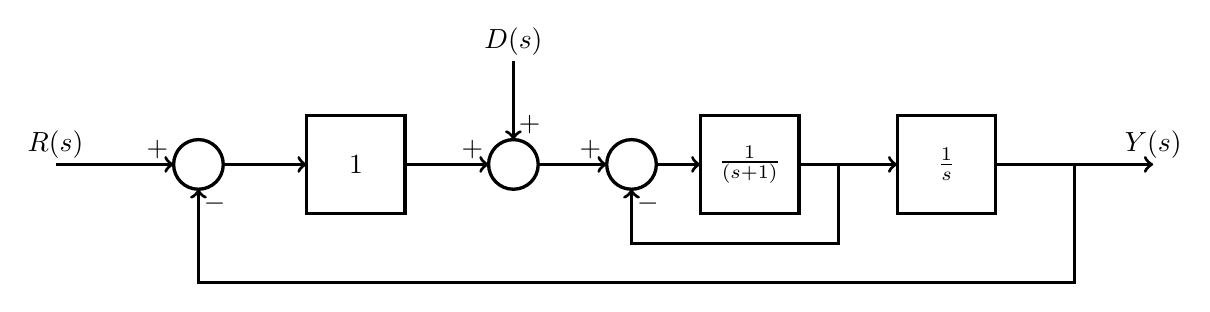
\begin{tikzpicture}[scale=1,inner sep=0pt,outer sep=0pt,very thick,
sysblock/.style={draw,rectangle,inner sep=4pt,minimum width=1.25cm,minimum height=1.25cm,very thick}]

\draw (-6,0) node[draw,circle] (sum1) {$\rule{0pt}{18pt}$};
\draw (-4,0) node[sysblock] (K) {1};
\draw (-2,0) node[draw,circle] (sum2) {$\rule{0pt}{18pt}$};
\draw (-.5,0) node[draw,circle] (sum3) {$\rule{0pt}{18pt}$};
\draw (1,0) node[sysblock] (G) {$\frac{1}{(s+1)}$};
\draw (3.5,0) node[sysblock] (G2) {$\frac{1}{s}$};
\draw[<-] (sum1.180) node[above left=2pt] {$+$} -- ++(-1.5,0) node[above=2pt] {$R(s)$};
\draw[->] (sum1.0) -- (K.180);
\draw[->] (K.0) -- (sum2.180) node[above left=2pt] {$+$};
\draw[<-] (sum2.90) node[above right=2pt] {$+$} -- ++(0,1) node[above=2pt] {$D(s)$};
\draw[->] (sum2.0) -- (sum3.180) node[above left=2pt] {$+$};
\draw[->] (sum3.0) -- (G.180);
\draw[->] (G.0) -- (G2.180);
\draw[->] (G.0) ++(0.5,0) -- ++(0,-1) -| (sum3.-90) node[below right=2pt] {$-$}; 
\draw[->] (G2.0) --  ++(2,0) node[above=2pt] {$Y(s)$};
\draw[->] (G2.0) -- ++(1,0) -- ++(0,-1.5) -| (sum1.-90) node[below right=2pt] {$-$};
\end{tikzpicture}
\end{center}